\documentclass{beamer}
\usetheme{Copenhagen}

\usepackage{siunitx}
\newcommand{\h}{\unit{\hour}}
\newcommand{\ph}{\unit{\per\hour}}
\newcommand{\um}{\unit{\micro\metre}}
\newcommand{\pums}{\unit{\per\micro\metre\squared}}
\newcommand{\nm}{\unit{\nano\mole\per\litre}}

\usepackage{amsmath}
\usepackage{amssymb}
\usepackage{cancel}
\usepackage{graphicx}
\graphicspath{{../images/}}

\title{An ODE Model of Root Zonation in \\ \emph{A. Thaliana} Mutants}
\author{Riley Wheadon}
\institute{University of British Columbia}
\date{November 20th, 2024}

\begin{document}

\frame{\titlepage}

\begin{frame}
\frametitle{Acknowledgements}
\begin{itemize}
  \item Dr. Eric Cytrynbaum (Supervisor)
  \item Dr. Geoffrey Wasteneys (Experimental Collaborator)
  \item NSERC USRA Program
\end{itemize}
\end{frame}

\begin{frame}
\frametitle{Root Zonation}
\begin{figure}
  \centering
  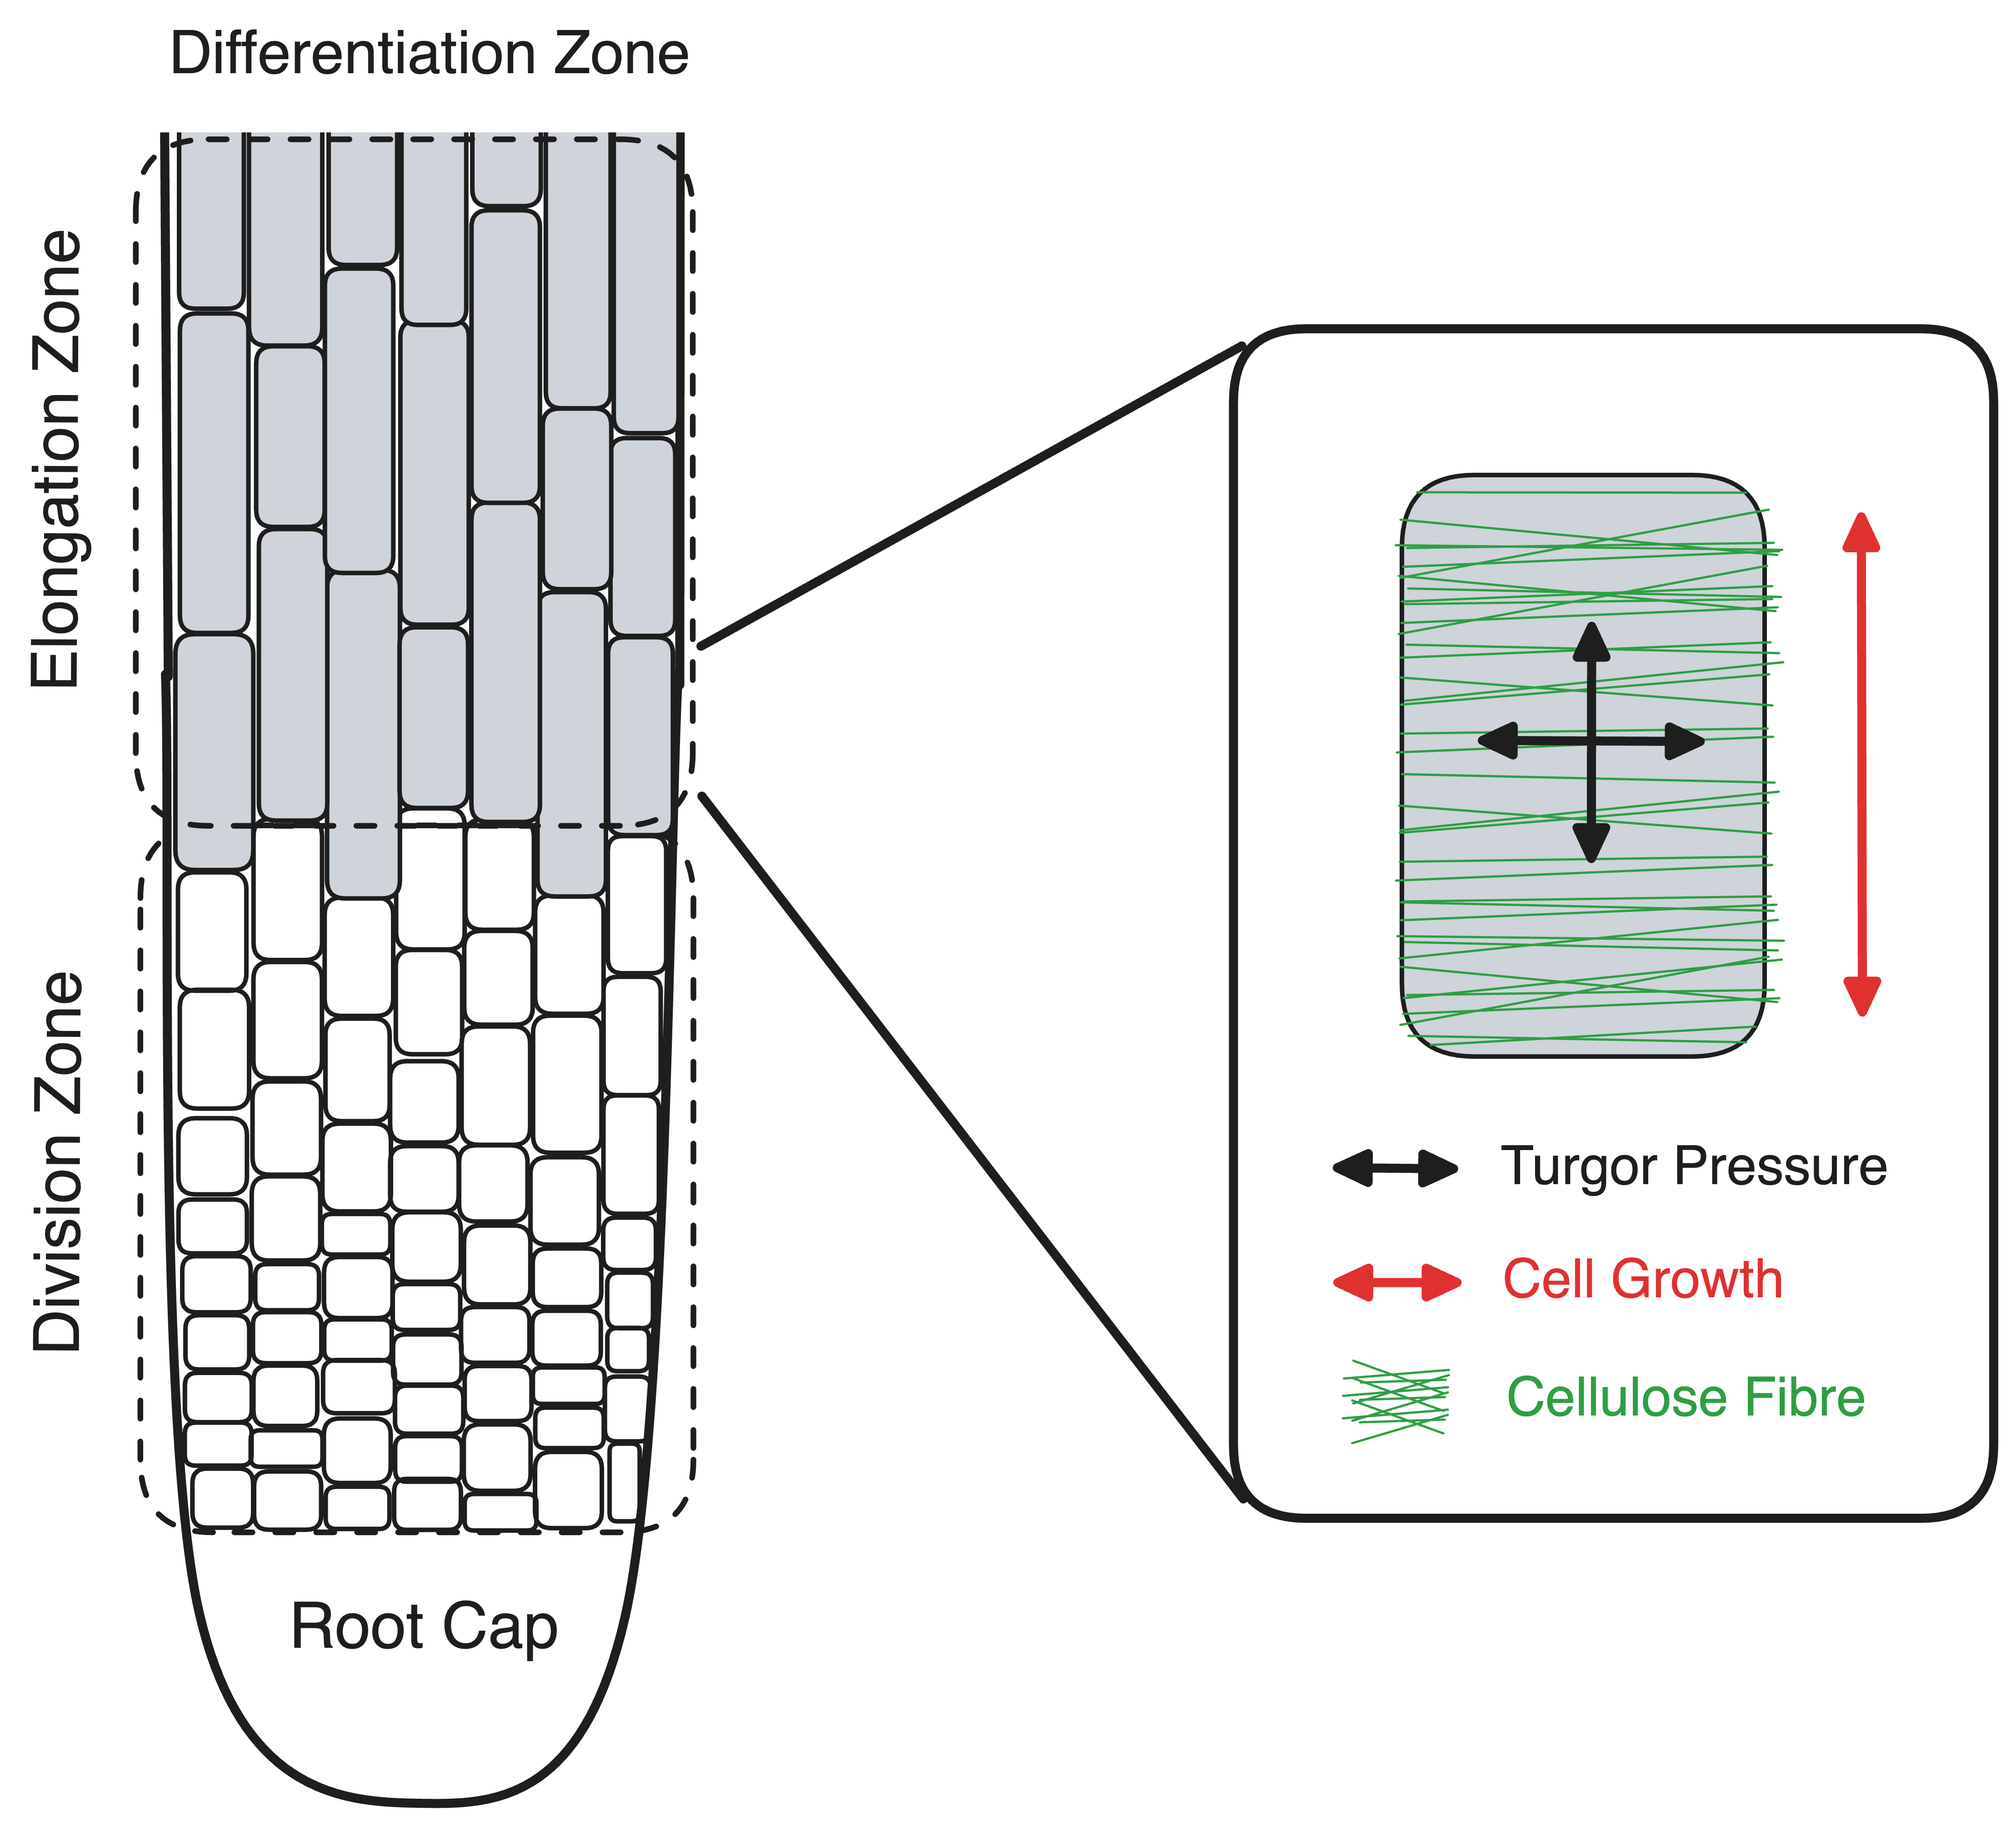
\includegraphics[height=16em]{root-zonation-simple.png}
  \caption{Zonation of the root apical meristem in \emph{A. thaliana}.}
\end{figure}
\end{frame}

\begin{frame}
\frametitle{Signalling Network}
\begin{figure}
  \centering
  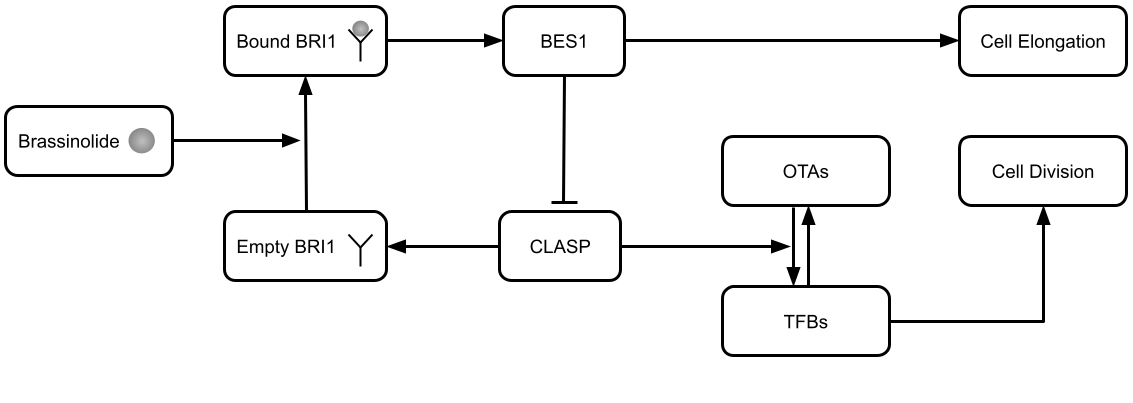
\includegraphics[width=\textwidth]{network-wild-type.png}
  \caption{Hormone interactions observed in \emph{A. thaliana} roots.}
\end{figure}
\end{frame}

\begin{frame}
\frametitle{\emph{brinCLASPpro} Mutant}
\begin{figure}
  \centering
  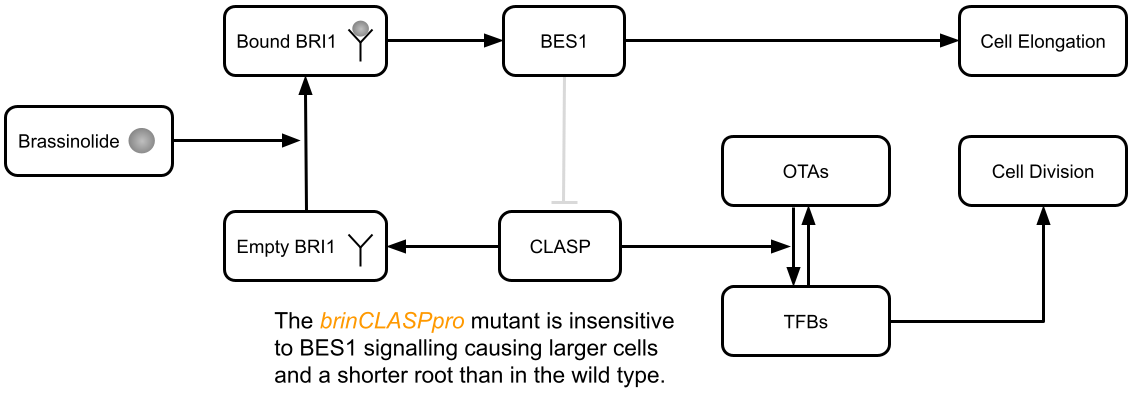
\includegraphics[width=\textwidth]{network-brin-clasp.png}
\end{figure}
\end{frame}

\begin{frame}
\frametitle{\emph{clasp-1} Mutant}
\begin{figure}
  \centering
  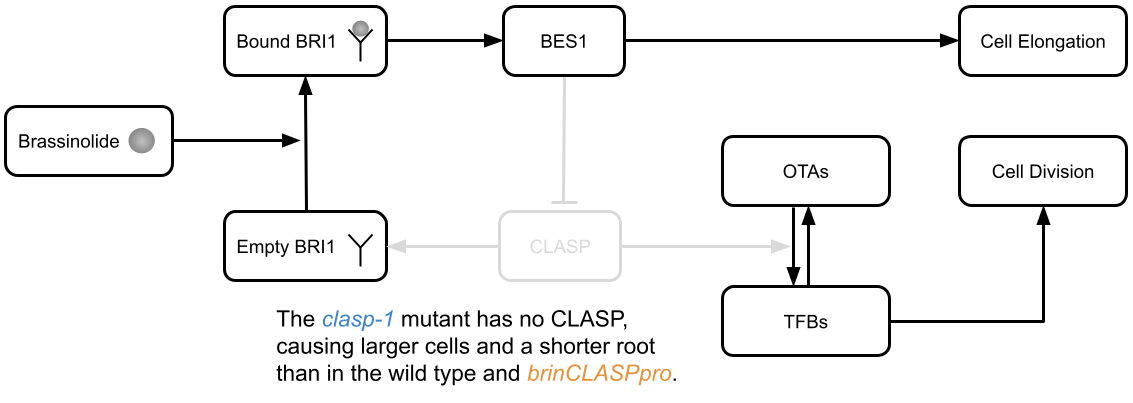
\includegraphics[width=\textwidth]{network-clasp-1.png}
\end{figure}
\end{frame}

\begin{frame}
\frametitle{Abridged Signalling Network}
\begin{figure}
  \centering
  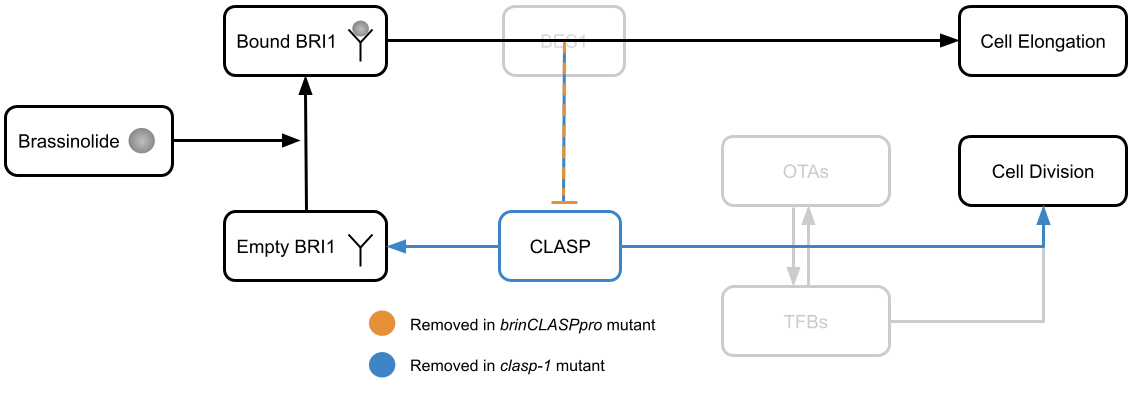
\includegraphics[width=\textwidth]{network-simplified.png}
  \caption{Simplified signalling network used in the model.}
\end{figure}
\end{frame}

\begin{frame}
\frametitle{Intracellular Model}

Since the intracellular signalling within the cell occurs faster than cell growth and division, we assume it is in a quasi-steady state.
$$
\begin{aligned}
  0 &= \frac{ dC }{ dt } = (c_{0} - c_{1}R_{B}) - c_{2}C \\[5pt]
  0 &= \frac{ dR_{T} }{ dt } = (r_{0}  + r_{1}C) - r_{2}R_{T} \\[5pt]
  R_{B} &= f(B, R_{T}, K_{d})
\end{aligned}
$$

\end{frame}

\begin{frame}
\frametitle{Extracellular Model}
Shown below are the equations for cell growth ($dL/dt$) and division ($dD/dt$). When $D = 1$, the cell divides into two cells with $D = 0$.
$$
\begin{aligned}
\frac{ dD }{ dt } &= (1 + \delta_{0}C) \left( 1 - \frac{ L^{ n } }{ \delta_{1}^{ n } + L^{ n } } \right)  \\[5pt]
\frac{ dL }{ dt } &= \left(\gamma_{0}  +  \gamma_{1}R_{B}\right)L  
\end{aligned}
$$
\end{frame}

\begin{frame}
\frametitle{Initial Results}
\begin{figure}
  \centering
  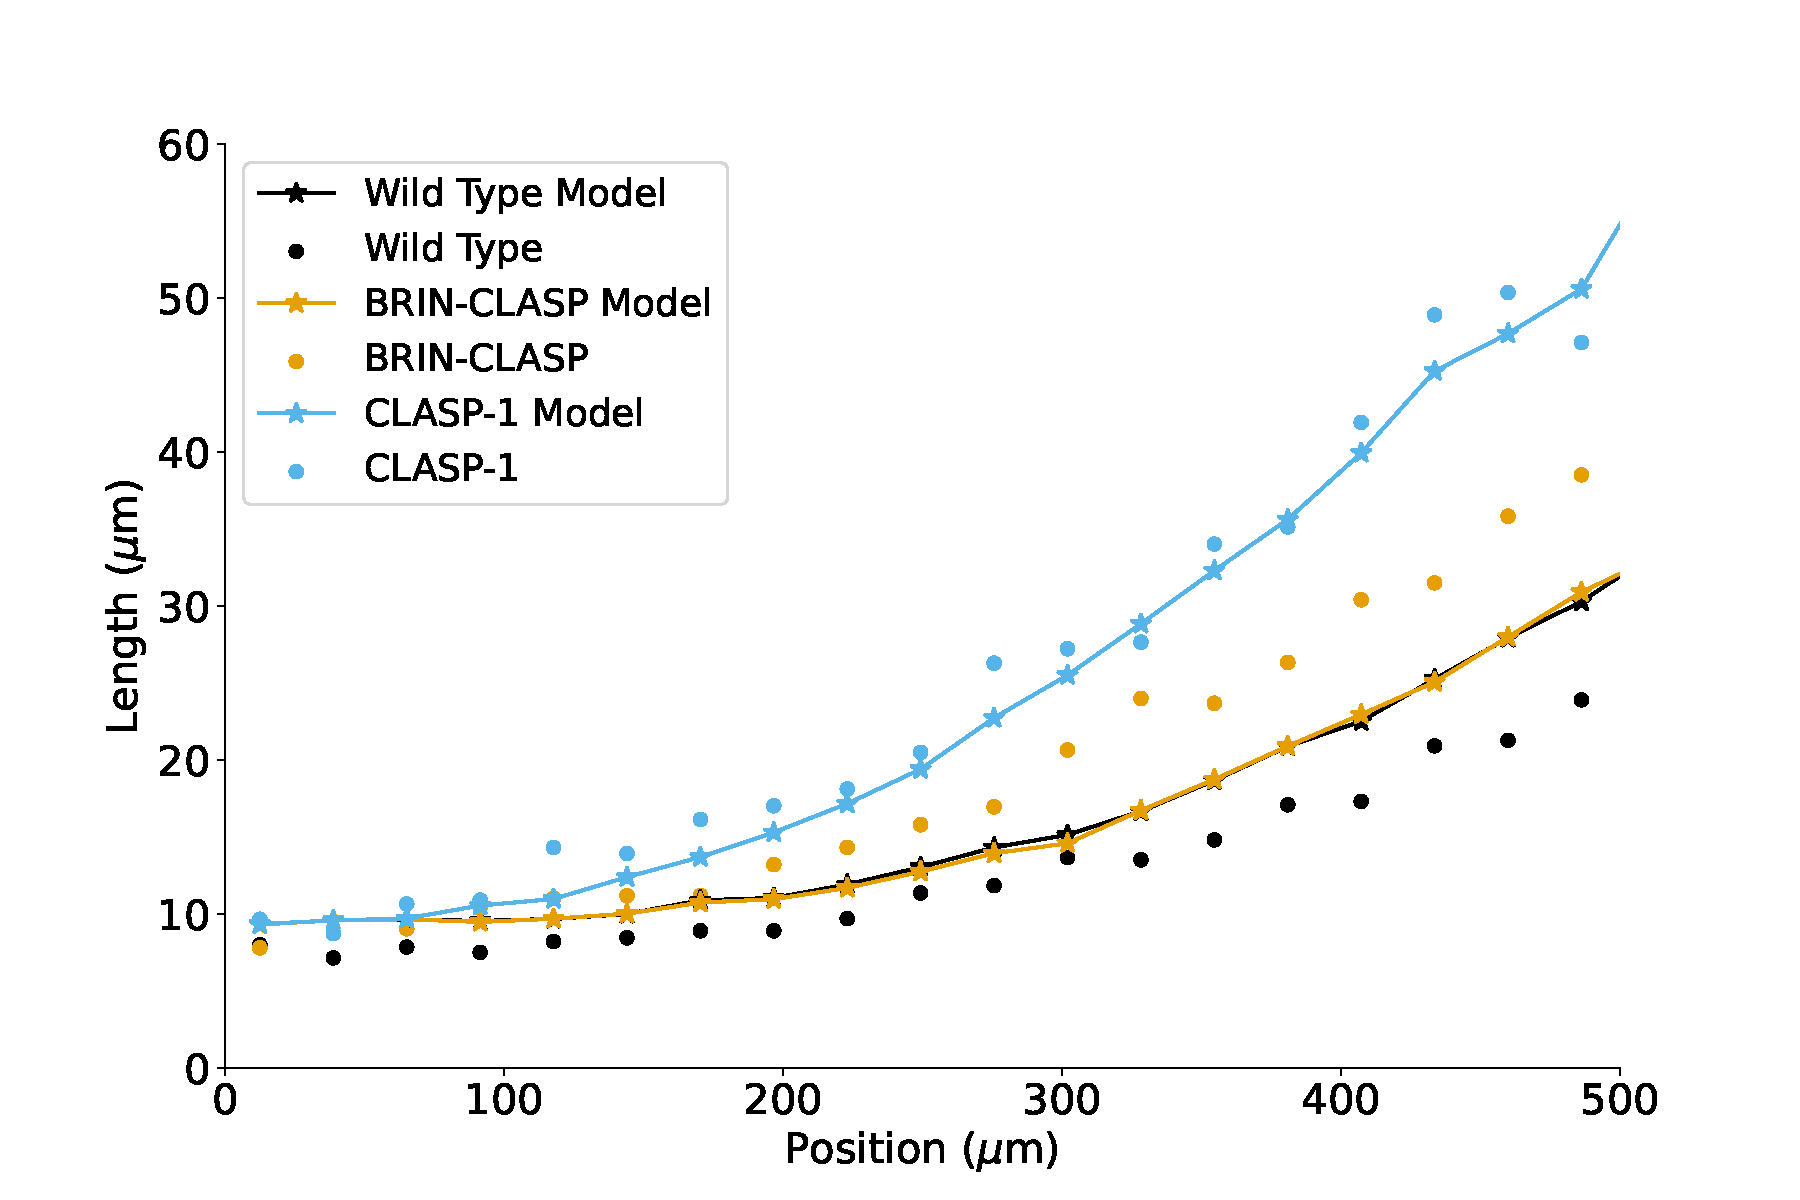
\includegraphics[height=16em]{column-original-fit.pdf}
  \caption{The model failed to differentiate cell lengths in the root apical meristem of the \emph{brinCLASPpro} mutant from the wild type.}
\end{figure}
\end{frame}

\begin{frame}
\frametitle{Explaining the \emph{brinCLASPpro} Mutant}
\onslide<1->{\textbf{Idea}: Inhibit division in the \emph{brinCLASPpro} mutant relative to the wild type in order to increase cell length. We hypothesize this is caused by an excess of CLASP.}

\bigskip

\onslide<2->{
To implement this change, we modify the division equation:
$$
\frac{ dD }{ dt } = (\color{red}\sigma_{0} + \sigma_{1}C - C^{2}\color{black})\left(1 - \frac{ L^{ n } }{ \delta_{1}^{ n } + L^{ n } }\right)
$$}
 
\end{frame}

\begin{frame}
\frametitle{Updated Results (1/2)}
\begin{figure}
  \centering
  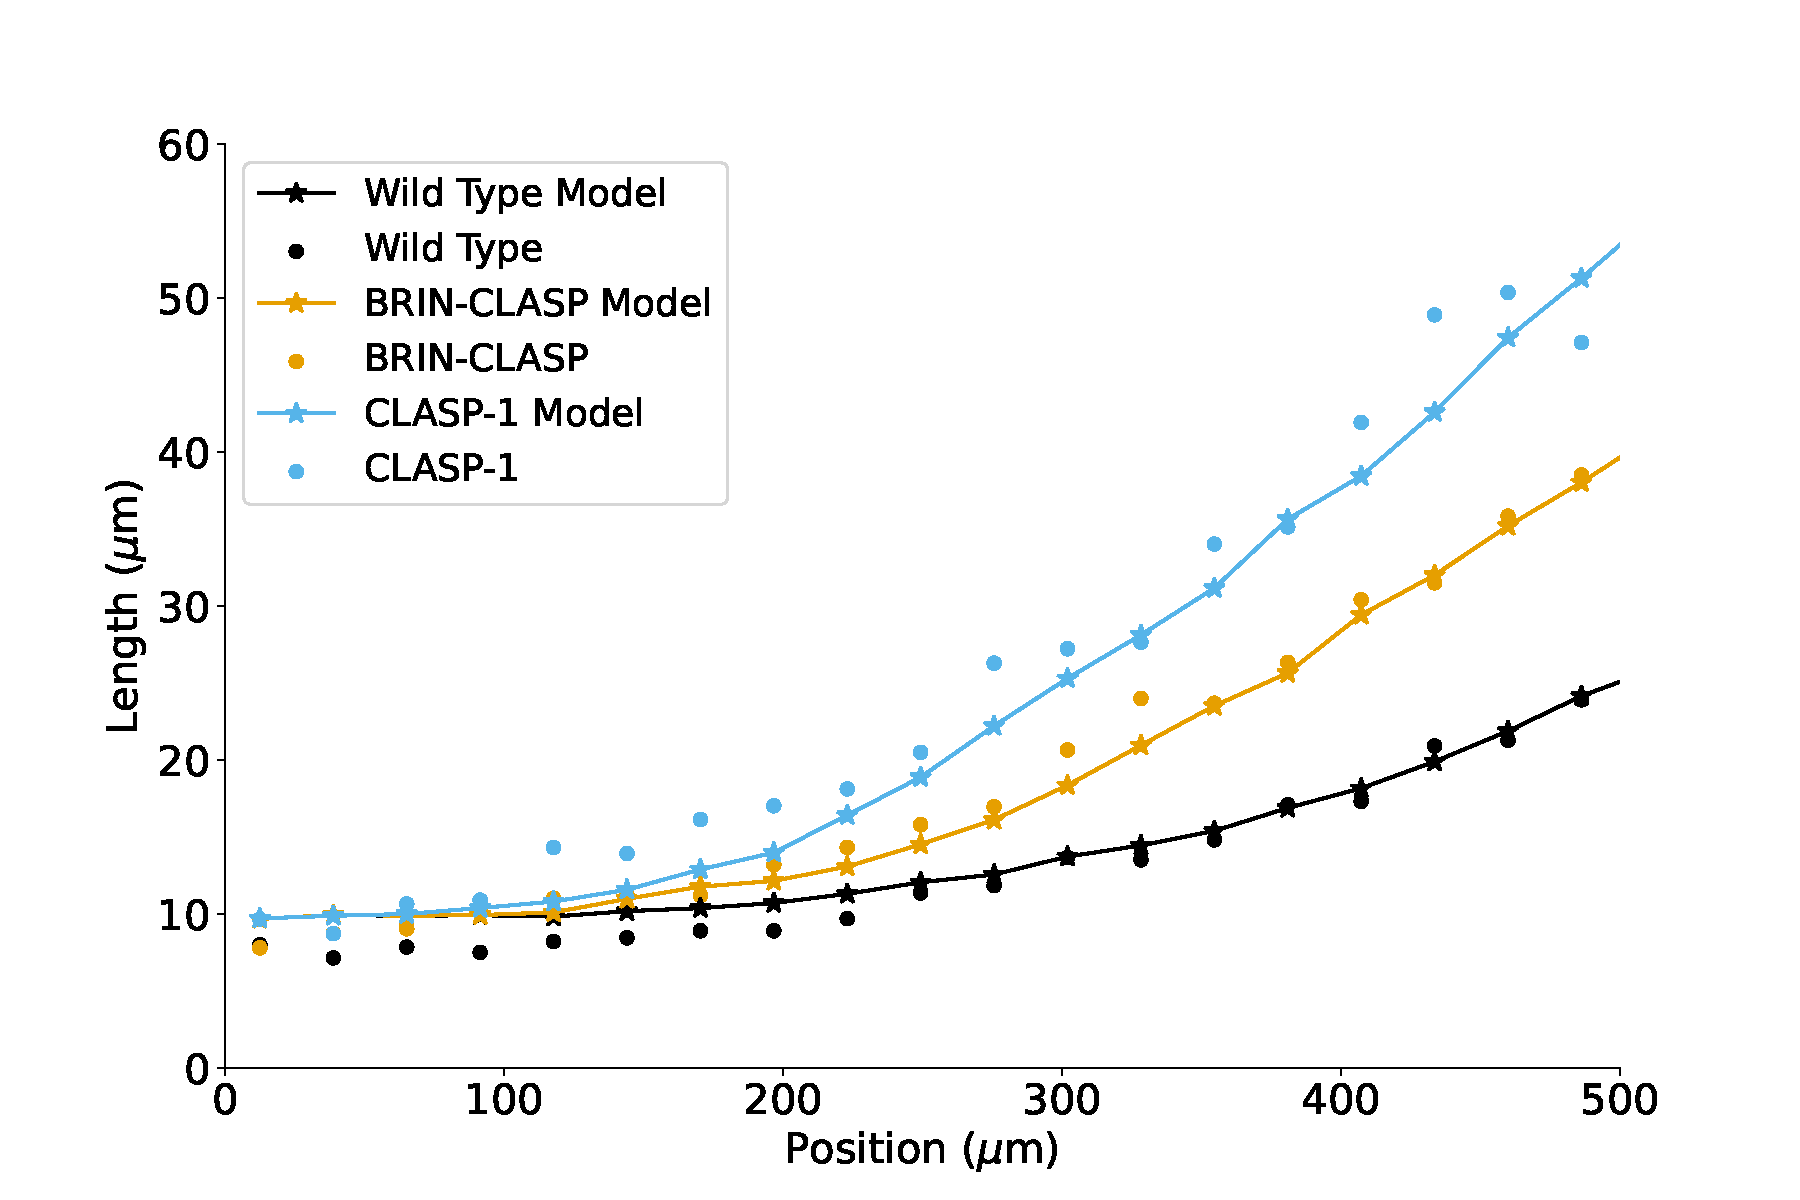
\includegraphics[height=16em]{column-modified-fit.pdf}
  \caption{The updated model correctly differentiates cell lengths in the \emph{brinCLASPpro} mutant from the wild type.}
\end{figure}
\end{frame}

\begin{frame}
\frametitle{Updated Results (2/2)}
The updated model accurately explains the mutant phenotypes:
\begin{center}
\medskip
\begin{tabular}{|c c c c |} 
 \hline
 Mutant & Length & Division Zone Size & Divisions  \\ [0.5ex] 
 \hline
 Wild Type & $43\,692\um$ &  $456.5\um$ & $324$ \\ 
 \hline
 \emph{brinCLASPpro} & $28\,352\um$ &  $275.0\um$ & $213$ \\
 \hline
 \emph{clasp-1} & $19\,241\um$ &  $234.5\um$ & $142$ \\
 \hline
\end{tabular}
\end{center}
\end{frame}

\begin{frame}
\frametitle{Conclusion}

\onslide<1->{\textbf{Key Idea}: A mechanism which causes the CLASP protein to inhibit cell division at superphysiological concentrations is sufficient to explain the \emph{brinCLASPpro} mutant.}

\bigskip

\onslide<2->{\textbf{Next Steps:}}
\begin{itemize}
 \item<2-> Integrating this work with intracellular microtubule models.
 \item<2-> Modelling the effects of CLASP on auxin signalling.
\end{itemize}

\bigskip

\onslide<3->{Thanks for listening. Any questions?}

\end{frame}

\end{document}


